\chapter{Dimensionality Reduction and Representation}
\label{ch:dimred}

\chapterguide%
  {\chapref{ch:unsupervised}, correlation and dot products from \chapref{ch:foundations}, and scaling from \chapref{ch:data}. Eigenvectors and eigenvalues are introduced here from scratch.}
  {explain PCA as choosing the best shadow; score a direction by hand; compute shares of variance; read a component's weights; choose how many components to keep from evidence; and read t-SNE and UMAP maps with care.}

The tutor wants all four columns of the study log on one chart. A chart has two axes, and the table has four columns, so that chart cannot be drawn. But you have known the way out since you were a child.

\section{The idea: find the best shadow}

\begin{analogy}
Hold a toy horse up to a lamp, and its shadow on the wall flattens three dimensions into two. Turn the horse side-on and the shadow keeps the head, legs and tail, spread out and recognizable. Turn it head-on and the shadow is a narrow blob. Same object, same lamp; the angle is everything. A \term{projection} is that flattening, and \term{principal component analysis (PCA)} finds the angle whose shadow keeps the most.
\end{analogy}

What does ``keeps the most'' mean as a number? In the good shadow, parts of the horse land far apart. In the bad one, everything lands on top of everything else. So we score a shadow by how spread out it is, and we already have a number for spread: the variance. PCA turns ``keep as much information as possible'' into ``keep as much variance as possible.''

\begin{utpfig}[Principal axes]{Principal component analysis finds better axes. The first component points along the direction of most variance; the second is perpendicular to it.}{fig:pca-axes}
\begin{tikzpicture}
\begin{axis}[
  width=0.80\linewidth, height=6.2cm,
  axis lines=middle,
  xlabel={$x_1$}, ylabel={$x_2$},
  ticks=none, xmin=-2.9, xmax=2.9, ymin=-2.7, ymax=2.7,
  clip=false
]
\addplot[only marks, mark=*, mark size=1.6pt] coordinates {
  (-2,-1.6) (-1.4,-1.1) (-0.6,-0.2) (0,0.3) (0.7,0.4)
  (1.3,1.2) (2,1.7) (-0.2,-0.5) (1.7,1.9) (-1.8,-2.0)
};
\draw[-{Stealth[length=2.4mm]}, very thick]
  (axis cs:0,0) -- (axis cs:2.0,1.6)
  node[right, font=\small] {PC1: most variance};
\draw[-{Stealth[length=2.4mm]}, thick]
  (axis cs:0,0) -- (axis cs:-0.64,0.8)
  node[above, font=\small] {PC2};
\end{axis}
\end{tikzpicture}
\end{utpfig}

\section{One shadow by hand}

Start with two columns: hours studied and hours slept. Their correlation is $-0.96$, so they are nearly one story told twice. Scale each column to mean 0 and standard deviation 1 first, because we are about to add hours of study to hours of sleep, and each column should get an equal voice. Student J, for example, becomes $(1.57,\,-1.85)$: well above average on study, well below on sleep.

Now pick a direction, written as weights whose squares add to 1, so that one step along it has length 1. The direction $(0.71,-0.71)$ means ``study up, sleep down.'' A student's shadow on that line is a dot product: J's is $0.71\times1.57+(-0.71)\times(-1.85)\approx2.4$, far along the line.

\begin{workedexample}
Take the shadow of all ten students on two perpendicular directions, and compute the variance of each set of shadows.

\medskip
\centering\small
\begin{tabular}{@{}lcc@{}}
\toprule
\rowcolor{UTPPaleBlue!92}
\utpth{Direction} & \utpth{Meaning} & \utpth{Spread of the shadows} \\
\midrule
$(0.71,-0.71)$ & study up, sleep down & 1.965 \\
$(0.71,\ 0.71)$ & study and sleep up together & 0.035 \\
\bottomrule
\end{tabular}
\par\raggedright
\medskip
The two scaled columns hold 2 units of spread in total, and one direction holds 1.965 of them, or 98\%. The students barely differ at all along the other. Nothing would be lost by replacing these two columns with one new column, ``cramming versus resting.''
\end{workedexample}

\begin{utpfig}[Two shadows of the same students]{Hours and sleep, both scaled. Along the ``study up, sleep down'' direction the students spread out, keeping 1.965 of the 2 units of spread. Along the perpendicular direction they crowd together, keeping 0.035.}{fig:shadow}
\begin{tikzpicture}
\begin{axis}[logaxis, width=7.6cm, height=7.0cm, axis equal image, xmin=-2.4, xmax=2.4, ymin=-2.4, ymax=2.4, xlabel={hours, scaled}, ylabel={sleep, scaled}]
\addplot[draw=UTPBlue,thick,domain=-2.2:2.2] {-x};
\addplot[draw=UTPOrange,thick,dashed,domain=-2.2:2.2] {x};
\addplot[only marks,mark=*,mark size=1.9pt,draw=UTPNavy,fill=UTPNavy] coordinates {(-1.57,1.15)(-1.22,1.15)(-0.87,0.65)(-0.52,0.65)(-0.17,0.65)(0.17,0.15)(0.52,-0.35)(0.87,-0.85)(1.22,-1.35)(1.57,-1.85)};
\node[font=\scriptsize\color{UTPBlue},anchor=south west] at (axis cs:0.9,-1.0) {spread 1.965};
\node[font=\scriptsize\color{UTPOrange!85!black},anchor=south east] at (axis cs:1.7,1.7) {spread 0.035};
\end{axis}
\end{tikzpicture}
\end{utpfig}

\section{All four columns at once}

PCA runs the same scoring over every possible direction, using one piece of mathematics. Doing the correlation for every pair of columns fills a table; on scaled data it is also the covariance table.

\begin{utptable}
\centering
\begin{tabular}{@{}lcccc@{}}
\toprule
\rowcolor{UTPPaleBlue!92}
\utpth{} & \utpth{hours} & \utpth{lectures} & \utpth{sleep} & \utpth{mark} \\
\midrule
hours & 1.00 & $-0.15$ & $-0.96$ & $-0.25$ \\
lectures & $-0.15$ & 1.00 & 0.35 & 0.86 \\
sleep & $-0.96$ & 0.35 & 1.00 & 0.46 \\
mark & $-0.25$ & 0.86 & 0.46 & 1.00 \\
\bottomrule
\end{tabular}
\end{utptable}

The \term{eigendecomposition} takes that table and returns every direction ranked by spread. Its two words name things we already have: an \term{eigenvector} is one direction, written as its weights, and its \term{eigenvalue} is that direction's spread. In formula form, $S\bm{v}=\lambda\bm{v}$: multiplying the table by the direction only stretches it. NumPy calls the routine \texttt{eigh}.

\lstinputlisting[style=utppython,firstline=108,lastline=114]{all_experiments/demo_study_log.py}

\begin{workedexample}
The four directions have spreads 2.532, 1.330, 0.130 and 0.008, out of 4 units in total. Their shares are 63.3\%, 33.2\%, 3.3\% and 0.2\%. So the first two together keep 96.5\%, and the other two can go.

\medskip
\centering\small
\begin{tabular}{@{}lccccl@{}}
\toprule
\rowcolor{UTPPaleBlue!92}
\utpth{Direction} & \utpth{hours} & \utpth{lectures} & \utpth{sleep} & \utpth{mark} & \utpth{What it reads as} \\
\midrule
PC1 & $-0.48$ & 0.46 & 0.56 & 0.50 & attending and rested, not cramming \\
PC2 & 0.56 & 0.55 & $-0.40$ & 0.47 & how much work went in \\
\bottomrule
\end{tabular}
\par\raggedright
\medskip
A big weight means the column matters, and the signs show which columns move together. The names are ours, read from the weights. The sign of a whole direction is arbitrary, so software may flip it.
\end{workedexample}

Multiplying the scaled table by those two directions gives every student two new coordinates, and the whole group finally fits on one chart (\figref{fig:pc-map}). Far right are D, E and F, who attended, slept and did well. Far left are I and J, the crammers. At the bottom are A and B, who did little work, and at the top are F and G, who did a lot. The three groups $K$-means found from only hours and mark in \chapref{ch:clustering} land in three separate regions, and this time the map also used lectures and sleep. That is the check we promised: the crammers really are the students who skipped lectures and barely slept.

\begin{utpfig}[The whole group on one chart]{Each student on the first two principal components, keeping 96.5\% of the spread of all four columns. Markers show the groups $K$-means found from hours and mark alone.}{fig:pc-map}
\begin{tikzpicture}
\begin{axis}[logaxis, width=0.72\linewidth, height=6.2cm, xlabel={PC1: attending and rested, not cramming}, ylabel={PC2: work put in}, xmin=-4, xmax=2.4, ymin=-2.5, ymax=2.5,
  legend style={at={(0.03,0.97)},anchor=north west},
  nodes near coords, point meta=explicit symbolic,
  every node near coord/.append style={font=\tiny\bfseries\color{UTPNavy},anchor=south,inner sep=1.5pt}]
\addplot[only marks,mark=*,mark size=2pt,draw=UTPBlue,fill=UTPBlue] coordinates {(0.93,-1.78)[A] (0.59,-1.83)[B] (0.69,-0.88)[C]};
\addlegendentry{light studiers}
\addplot[only marks,mark=square*,mark size=2pt,draw=UTPOrange,fill=UTPOrange] coordinates {(1.09,-0.08)[D] (1.35,0.60)[E] (1.60,1.72)[F] (0.35,1.33)[G]};
\addlegendentry{steady}
\addplot[only marks,mark=triangle*,mark size=2.4pt,draw=UTPGreen,fill=UTPGreen] coordinates {(-0.83,0.95)[H] (-2.41,0.07)[I] (-3.38,-0.10)[J]};
\addlegendentry{crammers}
\end{axis}
\end{tikzpicture}
\end{utpfig}

\recipecard{PCA}{A set of directions to flatten the data onto.}{The spread lost by flattening: here 3.5\% with two directions.}{An exact matrix routine, the eigendecomposition or the SVD, which finds every direction at once.}

\section{PCA step by step}

\begin{enumerate}
  \item \term{Center} the data by subtracting each feature's training mean. Decide separately whether to standardize: do so when equal standardized variation should carry equal weight, but retain original units when their variance is scientifically meaningful.
  \item Compute the sample covariance matrix
  \[
    S=\frac{1}{n-1}X^{\mathsf T}X
  \]
  for the centered matrix $X$.
  \item Find its eigenvectors and eigenvalues: for centered data matrix $X$,
  \[
    S\bm{v}=\lambda\,\bm{v}.
  \]
  Each eigenvector $\bm{v}$ is a component direction; its eigenvalue $\lambda$ measures the variance captured along it.
  \item \term{Sort} components by eigenvalue and keep the top $k$.
  \item \term{Project}: the new features (\term{scores}) are the dot products of each observation with the kept components.
\end{enumerate}

The proportion of variance explained by component $j$ is
\[
  \frac{\lambda_j}{\sum_{k}\lambda_k},
\]
explaining the variance along each axis, not its predictive value (\secref{sec:pca-limitations}). Components are orthogonal and fitted scores uncorrelated. SVD of centered data computes the same directions.

\begin{workedexample}
Take five centered points that lie exactly on a line: $(-2,-2)$, $(-1,-1)$, $(0,0)$, $(1,1)$, $(2,2)$. Each feature has variance $10/4=2.5$ and their covariance is also $2.5$, so the covariance matrix is
$\begin{bsmallmatrix}2.5 & 2.5\\ 2.5 & 2.5\end{bsmallmatrix}$
with $\lambda_1=5$, $\lambda_2=0$, and $\bm v_1=(1,1)/\sqrt2$. Scores $(-2.83,-1.41,0,1.41,2.83)$ retain 100\% of variance in one dimension. Dropping nonzero components instead loses variance.
\end{workedexample}

\section{Explained variance: the compression budget}

Lab~4 applies this to 8$\times$8 handwritten digits, 64 pixel columns per image. The first component alone keeps 14.9\%, and the first ten keep 74.1\%. Keeping 90\%, 95\% and 99\% of the variance needs 21, 29 and 41 components. What the last components hold is mostly pixel noise, and a downstream classifier proves it: logistic regression on all 64 pixels and on 29 components scores the same 0.9477 on the test file.

\begin{utpfig}[Cumulative explained variance]{Real numbers from Lab~4's training digits. Left: the share of variance per component for the first ten. Right: the cumulative share. The curve bends early: 29 of 64 components already keep 95.4\%.}{fig:cumulative-variance}
\begin{tikzpicture}
\begin{groupplot}[group style={group size=2 by 1,horizontal sep=1.3cm},
  logaxis, width=7.4cm, height=4.5cm]
\nextgroupplot[title={Variance per component},xlabel={component},ylabel={share of variance},ybar,bar width=7pt,ymin=0,ymax=0.17,xmin=0.3,xmax=10.7,xtick={1,...,10},yticklabel style={/pgf/number format/fixed},grid=none,ymajorgrids]
\addplot[fill=UTPPaleBlue,draw=UTPBlue] coordinates {(1,0.149)(2,0.134)(3,0.117)(4,0.084)(5,0.057)(6,0.051)(7,0.047)(8,0.037)(9,0.035)(10,0.031)};
\nextgroupplot[title={Cumulative variance kept},xlabel={number of components},ylabel={share kept},ymin=0,ymax=1.05,xmin=0,xmax=66]
\addplot[draw=UTPBlue,mark=*,mark size=1.3pt,thick] coordinates {(1,0.149)(2,0.283)(3,0.400)(4,0.484)(5,0.541)(8,0.675)(10,0.741)(15,0.837)(21,0.904)(29,0.954)(41,0.990)(50,0.999)(64,1.000)};
\draw[UTPOrange,thick,dashed] (axis cs:29,0) -- (axis cs:29,0.954);
\node[font=\scriptsize\color{UTPNavy},anchor=north west] at (axis cs:30,0.80) {29 components: 95.4\%};
\end{groupplot}
\end{tikzpicture}
\end{utpfig}

Choose the count by a variance target, a bend in the curve, or downstream validation on training folds. Discarded eigenvalues add up to the variance you lost: here 4.6\% for 29 components.

\begin{workedexample}
How few can you keep? On Lab~4's validation split, logistic regression scores 0.608 on 2 components, 0.868 on 5, 0.934 on 10, 0.954 on 29 and 0.955 on all 64. Two components make a fine picture and a poor classifier; twenty-nine are almost free.
\end{workedexample}

\subsection{What PCA cannot promise}
\label{sec:pca-limitations}

\begin{itemize}
  \item It is \term{linear}: a spiral or a curved sheet of data has structure PCA cannot straighten out.
  \item It is \term{scale-sensitive}: changing units changes the covariance matrix. Standardize when that influence is arbitrary, not as an automatic rule.
  \item \term{Variance is not predictive importance}: low-variance directions may carry label signal. LDA instead seeks class separation (\chapref{ch:classification}).
  \item \term{Interpretation}: inspect component weights; each component blends original features.
\end{itemize}

\begin{workedexample}
\textbf{Scale.} Run PCA on the raw study log, without scaling. The first direction then takes 80.2\% of the variance with a weight of 0.96 on the mark. It has found ``the column with the largest numbers'', since marks vary far more than hours of sleep. On scaled columns the first direction keeps 63.3\% and uses all four columns about equally. Neither is wrong; they answer different questions, so choose on purpose.
\end{workedexample}

\begin{pitfall}
Projecting a four-feature clustering into two PCA dimensions only visualizes its existing assignments. Clustering the two PCA columns instead is a different model with reduced information.
\end{pitfall}

\section{t-SNE and UMAP: maps for the eye}
\label{sec:tsne-umap}

For two-dimensional neighborhood maps rather than global variance preservation, consider t-SNE or UMAP.

\term{t-SNE} converts distances into neighbor probabilities and arranges points in 2-D so that neighborhoods are preserved: points close in the original space stay close on the map. Its main hyperparameter, \term{perplexity}, roughly sets the neighborhood size being honored (typical values 5--50).

\term{UMAP} pursues the same goal with different mathematics; it is much faster, tends to preserve somewhat more of the global arrangement, and --- unlike classic t-SNE --- can place \emph{new} points onto an existing map.

Both need cautious reading:

\begin{itemize}
  \item cluster sizes, empty gaps, and distances between separated groups can be artifacts; even apparent neighborhoods should be checked against original-space distances;
  \item check whether the interpretation survives changes in seeds and hyperparameters;
  \item for ordinary preprocessing PCA is the simpler default, because it can project new rows.
\end{itemize}

\begin{utptable}
\begin{tabular}{@{}p{0.3\linewidth}p{0.27\linewidth}p{0.31\linewidth}@{}}
\toprule
\rowcolor{UTPPaleBlue!92}
\utpth{} & \utpth{PCA} & \utpth{t-SNE / UMAP} \\
\midrule
Preserves & global variance, linear structure & local neighborhoods \\
Handles new points & yes (a projection) & UMAP yes; t-SNE awkwardly \\
Best use & preprocessing, compression, denoising & exploratory visualization \\
\bottomrule
\end{tabular}
\end{utptable}

PCA, t-SNE, and UMAP \term{extract} new features; \term{selection} retains original columns (\secref{sec:feature-selection}).

\begin{keyidea}
PCA quantifies lost variance; nonlinear maps emphasize neighborhoods and need cautious interpretation. A visualization is evidence to investigate, not a substitute for the original data.
\end{keyidea}

\begin{modelcard}{Dimensionality Reduction - Quick Guide}
\begin{tabularx}{\linewidth}{@{}>{\bfseries\leavevmode\color{UTPNavy}}p{0.24\linewidth}X@{}}
PCA is best for & Compressing correlated numerical features, denoising, visualization, and faster downstream modeling. \cr
Preprocessing & Center features; standardize when unit scales are arbitrary and equal standardized influence is intended. \cr
Main control & Number of components, by explained variance and validation. \cr
Visualization tools & t-SNE and UMAP make useful two-dimensional maps of neighborhoods. \cr
Watch for & Loss of interpretability, information loss, leakage from fitting on all data, and over-interpreting visual clusters. \cr
\end{tabularx}
\end{modelcard}

\begin{chapterrecap}
\begin{itemize}
  \item PCA is a shadow: it flattens rows onto the directions that keep the most spread.
  \item A direction is a list of weights, a shadow is a dot product, and the eigendecomposition of the correlation table ranks every direction at once.
  \item On the study log, two directions keep 96.5\% of four columns: four columns were really two stories.
  \item Choose the number of components from a variance target and a downstream test. On the digits, 29 of 64 lost nothing measurable.
  \item PCA is linear and sensitive to scale, and variance is not the same as usefulness for a label. t-SNE and UMAP make maps for looking at, not measuring on.
\end{itemize}
\end{chapterrecap}

\begin{quickcheck}
\begin{enumerate}
  \item What does PCA optimize when it chooses its first principal component?
  \item Two scaled columns have a correlation of 0.80. What spread does the direction $(0.71,0.71)$ keep, and what share of the total?
  \item PCA's first direction has weights near $0.25$ on four columns of very different meaning. What does that suggest?
  \item Why can standardization change which PCA directions appear most important?
  \item A model drops from 0.95 to 0.61 accuracy going from 29 components to 2, while the two-component plot looks clean. What should you conclude?
  \item Why should distances and apparent cluster sizes in a t-SNE or UMAP plot not be interpreted as exact properties of the original high-dimensional data?
\end{enumerate}
\end{quickcheck}

\begin{checkanswers}
\begin{enumerate}
  \item The variance of the shadows, among directions of length 1.
  \item For two scaled columns, the spreads are $1+r$ and $1-r$, so 1.80 of the 2 units, which is 90\%. Check against the study log: $r=-0.965$ gives 1.965 along $(0.71,-0.71)$.
  \item Each weight is small and similar, so that component is a general average of the columns, and no single column dominates it. Read the signs and any exceptions before naming it.
  \item Changing units changes each column's variance, and PCA chases variance, so the column with the largest numbers can win for no good reason.
  \item Two components are good for looking and not for predicting. A clean picture is not evidence of a good representation for the task.
  \item They are built to preserve local neighborhoods, so sizes and gaps between groups can be artifacts of the layout, and they change with seeds and settings.
\end{enumerate}
\end{checkanswers}

\labsection{4}{Unsupervised learning I: clustering and PCA}{sec:lab04-clustering-pca}

\begin{labproject}{Customer segments from two years of invoices, and a compressed view of 15,701 wood-defect images}
\textbf{Read first.} Chapters~\ref{ch:unsupervised}--\ref{ch:dimred}.\\
\textbf{Goal.} Turn raw invoice lines into one row per customer, find segments with K-means and DBSCAN and judge them by evidence and usefulness, then compress images with PCA and choose how much to keep by validation, testing once.\\
\textbf{Scenario.} An online gift shop hands you two years of invoices and asks who its customers are, with no labels to learn from. A sawmill's inspection camera photographs every defect on its boards and asks how much of each photo it really needs to keep. Neither question has an answer key, so the evidence has to come from the data and from what the answer is for.\\
\textbf{Data.} In \texttt{all\_datasets/}: \texttt{unsupervised/\allowbreak online\_retail\_ii/\allowbreak online\_retail\_ii.zip}, every invoice line of a UK online shop from December 2009 to December 2011, from the UCI repository (Chen, 2012); and \texttt{unsupervised/\allowbreak wood\_surface\_defects/\allowbreak wood\_defects.npz}, 15,701 photos of seven kinds of defect on sawn boards, cut from a public industrial dataset (Kodytek, Bodzas and Bilik, 2022).\\
\textbf{Notebook.} \texttt{all\_experiments/\allowbreak lab04\_clustering\_pca/\allowbreak lab04\_clustering\_pca\_worked.ipynb}, with a README beside it.\\
\textbf{Hand in.} The executed notebook, \texttt{results/lab04/}, the saved PCA model and a short conclusion, as listed in the checklist at the end of this sheet.
\end{labproject}

\labroadmap{Your map of this lab}{
      A & Build customer rows, segment them with $K$-means, find outliers with DBSCAN & 2--6 \\
      B & Compress wood-defect images with PCA, choose the budget, test once and save & 7--11 \\
      Finish & Save the evidence; then cluster the defect images & 12--14 \\
      After & Your-turn tasks, expected findings, troubleshooting and the two checklists & --- \\
}

\begin{labmode}
\begin{enumerate}
  \item Activate your course environment and confirm the two data files are in \texttt{all\_datasets/}. Keep the ZIP file as it is: pandas reads the CSV inside it directly.
  \item From the course folder, start Jupyter, open the notebook, and choose \textbf{Restart Kernel and Run All Cells}. It takes about two minutes; the pixel models of Questions~8 and~9 take most of it.
  \item Part~A is clustering and Part~B is PCA. Neither has an answer key, so each question asks for the evidence a result needs.
\end{enumerate}
\begin{lstlisting}[style=utpterminal]
jupyter lab
\end{lstlisting}
Prefer a plain script? From the course folder, \texttt{python all\_experiments/\allowbreak lab04\_clustering\_pca/\allowbreak lab04\_clustering\_pca\_worked.py} runs the same code and writes the same evidence.
\end{labmode}

\labroutine

\begin{yourturn}
\textbf{Warm-up on paper.} Do these before opening the notebook; the code will check you.
\begin{enumerate}
  \item A customer bought on 1 November 2011 and on 2 December 2011, in two orders worth \pounds 120 and \pounds 80. The data ends on 9 December 2011, and recency is counted from the day after. What are this customer's recency, frequency and monetary value?
  \item Spend runs from \pounds 3 to \pounds 580,987, with a median of \pounds 868. Why would K-means on the raw numbers spend most of its effort on a few customers, and what does taking logs change?
\end{enumerate}
\end{yourturn}

\begin{labquestion}{1}{Setup}
Run this first, and keep this kernel for the later questions. Every lab starts the same way. \texttt{start\_lab()}, from \texttt{all\_experiments/\allowbreak course\_setup.py}, finds the course folder and returns the three folders the lab uses: \texttt{DATA} to read from, \texttt{RESULTS} and \texttt{MODELS} to write to. The imports in between are grouped by what they are for.
\end{labquestion}
\begin{labanswer}
\lstinputlisting[style=utppython,firstline=11,lastline=30]{all_experiments/lab04_clustering_pca/lab04_clustering_pca_worked.py}
\begin{refoutput}
\begin{lstlisting}[style=utpterminal]
course folder: MACHINE LEARNING
reads all_datasets/, writes results/lab04/ and models/
\end{lstlisting}
\end{refoutput}
\end{labanswer}

\labpartopen{Part A}{Clustering customers from their invoices}{Questions 2--6 \textbullet\ Data: Online Retail II invoices}{Turn a million invoice lines into one row per customer, then find segments with $K$-means and outliers with DBSCAN.}

\begin{labquestion}{2}{Build one row per customer}
Clustering needs one row per customer, and the file holds one row per invoice line. Clean the lines with fixed rules, then summarize each customer by recency (days since the last purchase), frequency (number of orders) and monetary value (total spend): the RFM table marketers use. All three have long right tails, so they are logged before scaling.
\end{labquestion}
\begin{labanswer}
\courselabtrace{Clustering and compression answer different questions}{K-means}{Assign each point to a nearest centroid}{DBSCAN}{Dense neighborhoods form clusters; noise may remain}{PCA}{Rotate onto variance directions; test reconstruction or utility}

\lstinputlisting[style=utppython,firstline=32,lastline=59]{all_experiments/lab04_clustering_pca/lab04_clustering_pca_worked.py}
\begin{refoutput}
\begin{lstlisting}[style=utpterminal]
invoice lines: 1067371  from 2009-12-01 to 2011-12-09
no customer ID: 0.228  cancellations: 0.018  exact duplicates: 34335
779425 clean lines from 5878 customers
      recency_days  orders     spend
50%           95.0     3.0     867.7
mean         200.9     6.3    2955.9
max          738.0   398.0  580987.0
\end{lstlisting}
\end{refoutput}

\textbf{What it means.} Over a million lines become 779,425 sales from 5,878 customers. Almost a quarter of the lines have no customer ID, so they cannot belong to anyone's history; cancellations, returns and repeated lines would distort the totals. Every rule is fixed, so it may run before any model. The mean spend is more than three times the median, the long tail the logs are there to tame.
\end{labanswer}

\begin{labquestion}{3}{Score $k$ from 2 to 8}
K-means needs $k$ in advance. Inertia always falls as $k$ grows, so look for a bend; the silhouette asks how much closer each customer is to its own cluster than to the next one, and peaks at a good $k$.
\end{labquestion}
\begin{labanswer}
\courselabtrace{Trace the actual customer segmentation}{1. Input / state}{Scale Age, Annual Income and Spending Score to form X.}{2. Operation}{KMeans uses five clusters and 30 initialisations; DBSCAN uses eps 0.75 and min\_samples 6.}{3. Check}{k\_labels assign K-means groups; d\_labels uses -1 for noise. profile reports original-unit means.}

\lstinputlisting[style=utppython,firstline=61,lastline=82]{all_experiments/lab04_clustering_pca/lab04_clustering_pca_worked.py}
\begin{labvisual}{Reference plot from the supplied notebook}
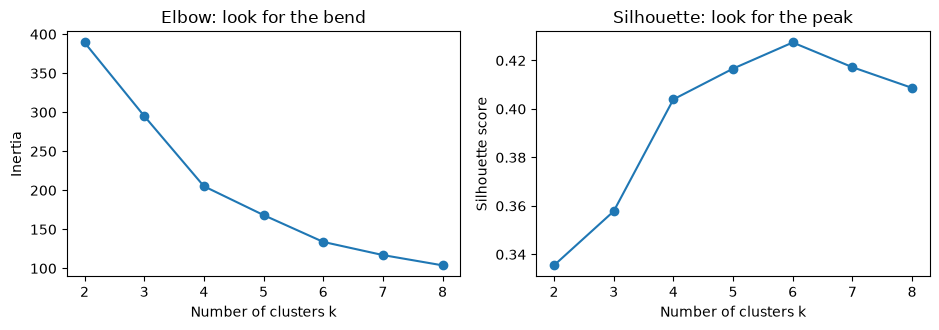
\includegraphics[width=.88\linewidth,height=5cm,keepaspectratio]{labs/visuals/04-notebook-reference.png}
\end{labvisual}
\begin{refoutput}
\begin{lstlisting}[style=utpterminal]
k=2  inertia=8600.4  silhouette=0.439
k=3  inertia=6375.8  silhouette=0.347
k=4  inertia=4963.7  silhouette=0.365
k=5  inertia=4137.7  silhouette=0.339
...
k=8  inertia=2919.8  silhouette=0.307
\end{lstlisting}
\end{refoutput}

\textbf{What it means.} The silhouette peaks at $k=2$, a split into active and inactive customers that any shopkeeper already knows. Among the richer splits, $k=4$ beats both 3 and 5. The numbers narrow the choice; what the segments are for decides it, and the next questions use four.
\end{labanswer}

\begin{labquestion}{4}{Compare K-means with DBSCAN}
K-means with four segments, against DBSCAN, which finds dense regions and leaves the rest as \emph{noise}. Here noise is not an error: it is the customers who look like no one else.
\end{labquestion}
\begin{labanswer}
\lstinputlisting[style=utppython,firstline=84,lastline=97]{all_experiments/lab04_clustering_pca/lab04_clustering_pca_worked.py}
\begin{refoutput}
\begin{lstlisting}[style=utpterminal]
K-means (k=4) silhouette: 0.365
DBSCAN clusters: 2  noise customers: 91  their share of revenue: 0.308
noise customers' median orders and spend: {'orders': 29.0, 'spend': 23419.0}
\end{lstlisting}
\end{refoutput}

\textbf{What it means.} DBSCAN finds two dense groups and refuses to place 91 customers, 1.5\% of them. Those 91 carry 30.8\% of the shop's revenue, with a median of 29 orders and \pounds 23,419: the wholesale buyers. A method allowed to say ``none of the above'' found the customers who matter most.
\end{labanswer}

\begin{labquestion}{5}{Describe the segments}
Medians describe each K-means segment in its own units, with its share of the shop's revenue.
\end{labquestion}
\begin{labanswer}
\lstinputlisting[style=utppython,firstline=99,lastline=109]{all_experiments/lab04_clustering_pca/lab04_clustering_pca_worked.py}
\begin{refoutput}
\begin{lstlisting}[style=utpterminal]
                customers  recency_days  orders   spend  revenue_share
kmeans_cluster
0                    2056         400.0     1.0   291.0          0.040
1                    1474         162.0     5.0  1587.0          0.179
2                    1117          15.0    13.0  5232.0          0.721
3                    1231          23.0     3.0   721.0          0.059
\end{lstlisting}
\end{refoutput}

\textbf{What it means.} Four segments a marketing team can act on: 2,056 lost one-time buyers who last ordered over a year ago; 1,474 lapsing regulars, worth a reminder; 1,231 recent occasional buyers, worth a second sale; and 1,117 best customers, who order every few weeks and bring in 72.1\% of all revenue. The cluster numbers are arbitrary; the names come from reading the medians.
\end{labanswer}

\begin{labquestion}{6}{Plot both clusterings}
Orders against spend, on log scales, colored by each method's labels.
\end{labquestion}
\begin{labanswer}
\lstinputlisting[style=utppython,firstline=111,lastline=124]{all_experiments/lab04_clustering_pca/lab04_clustering_pca_worked.py}

\textbf{What it means.} K-means cuts the cloud into four slices, because it always splits the space. DBSCAN draws a different line: its two dense clusters are simply the customers who ordered once and those who came back. Its noise points are the outliers, mostly at the top right, where a few customers have many orders and very large bills, plus a scattering of single unusually large orders.
\end{labanswer}

\begin{labcheckpoint}
\begin{itemize}[leftmargin=1.2em,itemsep=2pt,topsep=1pt]
  \item 779,425 clean lines from 5,878 customers.
  \item The silhouette peaks at $k=2$ (0.439); $k=4$ scores 0.365.
  \item DBSCAN leaves 91 customers as noise, and they bring 30.8\% of the revenue.
\end{itemize}
\end{labcheckpoint}

\labpartopen{Part B}{PCA on wood-defect images}{Questions 7--11 \textbullet\ Data: wood surface defects}{Compress 3,072 pixels with PCA, choose how much to keep on validation, and open the test images once.}

\begin{labquestion}{7}{Load the images}
The source holds 20,276 photos of sawn boards, collected for automated quality control, with a box around each defect. The course file holds 15,701 of those defects, cut out and shrunk to 32 by 32 colour pixels, in seven types. Most boards carry several defects, so whole boards go to one side of each split, development or test: a defect never meets its neighbour from the same board on the other side. The test images stay closed until Question~9.
\end{labquestion}
\begin{labanswer}
\lstinputlisting[style=utppython,firstline=126,lastline=150]{all_experiments/lab04_clustering_pca/lab04_clustering_pca_worked.py}
\begin{refoutput}
\begin{lstlisting}[style=utpterminal]
images: (15701, 32, 32, 3)  boards: 10358
per defect type: {'live knot': 3000, 'dead knot': 3000, 'resin': 3000, 'knot with crack': 2276,
 'crack': 2169, 'marrow': 1181, 'quartzity': 1075}
12567 development and 3134 test images; boards in both: 0
\end{lstlisting}
\end{refoutput}

\textbf{What it means.} Each image becomes a row of $32\times32\times3=3{,}072$ numbers. Neighboring pixels, and the three colours of one pixel, are strongly correlated: that redundancy is what PCA can remove. The types are not balanced, so the per-type recall in Question~9 matters as much as the accuracy.
\end{labanswer}

\textbf{Connect it to the chapter.} K-means and PCA both had no answer key, and from here on PCA is judged against one.
% Reused from chapters/14-how-unsupervised-learning-works.tex
\begin{labvisual}{Recall the chapter model}
\begin{labgraphic}
\begin{tikzpicture}[
  bx/.style={draw=UTPBlue,fill=UTPPaleBlue,rounded corners=2mm,text width=4.4cm,minimum height=1.2cm,align=center,font=\small\bfseries\color{UTPNavy}},
  arr/.style={-{Stealth[length=2.2mm]},thick,draw=UTPTeal}
]
\node[bx] (s) at (-4.3,0) {Supervised\\$X+y \longrightarrow$ predict $y$};
\node[bx] (u) at (4.3,0) {Unsupervised\\$X \longrightarrow$ discover structure};
\draw[arr] (s.east) -- node[above,font=\scriptsize\color{UTPMuted}]{remove the supplied label} (u.west);
\end{tikzpicture}
\end{labgraphic}\end{labvisual}


\begin{labquestion}{8}{Choose a PCA budget on validation}
How much variance to keep is a hyperparameter, so it is chosen on validation rows: a quarter of the development boards, split off the same way. Logistic regression on all 3,072 pixels is the reference; with that many inputs it needs up to 3,000 steps to converge.
\end{labquestion}
\begin{labanswer}
\lstinputlisting[style=utppython,firstline=152,lastline=170]{all_experiments/lab04_clustering_pca/lab04_clustering_pca_worked.py}
\begin{refoutput}
\begin{lstlisting}[style=utpterminal]
all 3,072 pixels: validation accuracy = 0.6168
90% variance:  21 components, validation accuracy = 0.5701
95% variance:  50 components, validation accuracy = 0.5919
99% variance: 248 components, validation accuracy = 0.6072
\end{lstlisting}
\end{refoutput}

\textbf{What it means.} Ninety per cent of the variance fits in just 21 directions, but those directions describe the light and colour of the wood more than the shape of a defect, and they score 0.570. The score climbs with the budget, and 99\%, 248 components, comes within a point of all 3,072 pixels. The budget is 99\%: a twelvefold compression for almost no loss.
\end{labanswer}

\begin{labquestion}{9}{Open the test images once}
The chosen budget, 99\% of the variance, is refit on all the development images and scored once on the test boards, beside logistic regression on all 3,072 pixels.
\end{labquestion}
\begin{labanswer}
\lstinputlisting[style=utppython,firstline=172,lastline=186]{all_experiments/lab04_clustering_pca/lab04_clustering_pca_worked.py}
\begin{refoutput}
\begin{lstlisting}[style=utpterminal]
FINAL TEST (3,134 images from boards never seen in development)
all 3,072 pixels accuracy: 0.6375
PCA components kept: 253  variance retained: 0.99
PCA -> logistic accuracy: 0.6331
recall per defect type: {'live knot': 0.56, 'dead knot': 0.69, 'resin': 0.73, 'knot with crack': 0.43,
 'crack': 0.72, 'marrow': 0.74, 'quartzity': 0.58}
\end{lstlisting}
\end{refoutput}

\textbf{What it means.} On boards never seen before, 253 components score 0.633 against 0.638 for every pixel: half a point for a model twelve times smaller in its inputs. Knots with cracks are the hardest type (recall 0.43), because they look like the knots they are; cracks, resin and marrow are found most often. A linear model on pixels stops near 64\%; Lab~7 asks whether a network that learns its own features can do better.
\end{labanswer}

\begin{labquestion}{10}{See what 99\% looks like}
Rebuild eight test images from 90\% and from 99\% of the variance to see what each keeps, and draw how the variance accumulates over the 3,072 directions.
\end{labquestion}
\begin{labanswer}
\lstinputlisting[style=utppython,firstline=188,lastline=220]{all_experiments/lab04_clustering_pca/lab04_clustering_pca_worked.py}
\begin{refoutput}
\begin{lstlisting}[style=utpterminal]
components for 50%, 80%, 90%, 95% and 99% of the variance: [2, 8, 21, 51, 253]
the first three components hold 0.624 of the variance
\end{lstlisting}
\end{refoutput}

\textbf{What it means.} Two directions hold half of the variance and three hold 62\%: mostly how light or dark, and how yellow, the wood is. Rebuilt from 21 components, a knot is a soft brown blur; from 253, its rings and cracks come back. Variance is not the same as usefulness: the directions that matter for telling defects apart are the faint ones, deep in the curve.
\end{labanswer}

\begin{labquestion}{11}{Save and reload the model}
Save the pipeline, reload it, and check that it still names the first test images.
\end{labquestion}
\begin{labanswer}
\lstinputlisting[style=utppython,firstline=222,lastline=229]{all_experiments/lab04_clustering_pca/lab04_clustering_pca_worked.py}
\begin{refoutput}
\begin{lstlisting}[style=utpterminal]
file size (MB): 6.26
predicted: ['knot with crack', 'knot with crack', 'dead knot', 'dead knot', 'knot with crack']
actual:    ['knot with crack', 'knot with crack', 'knot with crack', 'dead knot', 'knot with crack']
\end{lstlisting}
\end{refoutput}

\textbf{What it means.} Four of the five first test images are named correctly, and the miss is the confusion Question~9 predicted: a knot with a crack called a dead knot. The file holds the 253 components, each 3,072 numbers long, and the classifier: the price of compression is storing the directions.
\end{labanswer}

\begin{labcheckpoint}
\begin{itemize}[leftmargin=1.2em,itemsep=2pt,topsep=1pt]
  \item Keeping 99\% of the variance takes 248 components and scores 0.6072 on validation, against 0.6168 for all pixels.
  \item On the test boards: 0.6375 for all pixels and 0.6331 with 253 components.
\end{itemize}
\end{labcheckpoint}

\labpartopen{Finish}{Save the evidence, then try it yourself}{Questions 12--14}{Write the results folder, then extend the lab yourself before reading one worked solution.}

\begin{labquestion}{12}{Save the evidence}
Write the numbers above to the results folder. These files are regenerated on every run, so do not edit them by hand.
\end{labquestion}
\begin{labanswer}
\lstinputlisting[style=utppython,firstline=231,lastline=243]{all_experiments/lab04_clustering_pca/lab04_clustering_pca_worked.py}
\end{labanswer}

\labsubhead{Try it yourself}

\begin{labquestion}{13}{Try it yourself}
Cluster images without their labels. Reduce the Question~8 fitting images to 50 PCA components, run K-means with 7 clusters, one per defect type, and only then compare the clusters with the true types, with the adjusted Rand index and a table of what each cluster contains. Attempt it in this empty cell before reading the solution.
\end{labquestion}

\begin{labquestion}{14}{One solution}
The labels are used only after the clustering, to judge it. The average image of each cluster shows what K-means grouped by.
\end{labquestion}
\begin{labanswer}
\lstinputlisting[style=utppython,firstline=247,lastline=269]{all_experiments/lab04_clustering_pca/lab04_clustering_pca_worked.py}
\begin{refoutput}
\begin{lstlisting}[style=utpterminal]
adjusted Rand index against the true defect types: 0.129
         images most common type  purity
cluster
2          1570        dead knot    0.56
1          1630        live knot    0.46
3          1048            resin    0.39
...
0           380            resin    0.27
\end{lstlisting}
\end{refoutput}

\textbf{What it means.} The clusters barely match the types: an adjusted Rand index of 0.129, where 1 would be the types exactly and 0 a random split. The purest cluster is only 56\% dead knots. The average images show why: K-means grouped the defects by brightness, colour and the direction of the grain, which is what varies most in pixels, not by what a grader calls a defect. Without labels, ``similar'' means similar pixels.
\end{labanswer}

\labpartopen{After the lab}{Your turn, troubleshooting and hand-in}{Your-turn tasks \textbullet\ Expected findings \textbullet\ Troubleshooting \textbullet\ Checklists}{Extend the lab with the Your-turn tasks, compare with the expected findings, and check your work against the two checklists before you hand it in.}

\begin{yourturn}
Add new cells at the end of the notebook for these tasks, and record your numbers before reading the expected findings.
\begin{enumerate}
  \item \textbf{One start or many?} Rerun K-means on the customers at $k=4$ with \texttt{n\_init=1}, for seeds 0 to 7, and record each inertia. Then do the same for the Question~14 images at $k=7$. What does the difference say about \texttt{n\_init}?
  \item \textbf{Take the logs away.} Refit K-means at $k=4$ on the scaled but unlogged RFM columns, and compare the labels with Question~4's using \texttt{adjusted\_rand\_score}. How large are the four clusters?
  \item \textbf{Four or five?} Print the segment profile for $k=5$. Which of the four segments splits, and could a marketing team use that split?
  \item \textbf{How few components?} Score logistic regression on the Question~8 validation rows with 2, 10 and 50 components. What share of the variance do two components keep, and what are they good for?
\end{enumerate}
\end{yourturn}

\begin{expectedfindings}
\textbf{Warm-up.} Recency 8 days (from 2 December to 10 December), frequency 2, monetary value \pounds 200. On raw numbers a gap of \pounds 100,000 between two big spenders outweighs every other difference, so the few largest customers decide the clusters; logs measure spend in ratios, so \pounds 300 against \pounds 3,000 counts as much as \pounds 3,000 against \pounds 30,000.
\begin{enumerate}
  \item The customers are stable: all eight single starts end between 4,963.7 and 4,964.0. The images are not: eight starts end between 248,598 and 251,895, and only three of them land within a few units of the best. Four well-separated customer groups leave little room for a bad start, while seven overlapping defect groups in 50 dimensions leave plenty. Several starts cost little and protect against the second case.
  \item The adjusted Rand index against Question~4 is only 0.172, and the clusters hold 3,840, 1,999, 35 and 4 customers: two of the four ``segments'' are just the biggest spenders. Without the logs, the units decide the clustering.
  \item At $k=5$ the best customers split into 480 ``champions'' (median 7 days since the last order, 23 orders, \pounds 9,324) and 1,267 loyal regulars (35 days, 8 orders, \pounds 2,910). A team with a small budget for personal service may well want that split, an argument the silhouette alone cannot make.
  \item Validation accuracy is 0.420 with 2 components, 0.538 with 10 and 0.591 with 50, against 0.607 with 248. Two components keep 53.0\% of the variance, mostly the light and colour of the wood: good for drawing all the images on one page, not for telling a crack from a knot.
\end{enumerate}
\end{expectedfindings}

\begin{troubleshoot}
\begin{description}
  \item[\texttt{FileNotFoundError} for the ZIP] Keep \texttt{unsupervised/\allowbreak online\_retail\_ii/\allowbreak online\_retail\_ii.zip} zipped in \texttt{all\_datasets/}; pandas reads the CSV inside it.
  \item[A \texttt{KMeans} memory-leak warning on Windows] scikit-learn suggests setting \texttt{OMP\_NUM\_THREADS}; the results are unaffected.
  \item[Question~2 is slow] Reading a million lines takes a few seconds.
  \item[Questions~8 and~9 take a minute each] Logistic regression on 3,072 pixels needs many steps; \texttt{max\_iter=3000} lets it converge. With the default it stops early and warns.
\end{description}
\end{troubleshoot}

\begin{labchecklists}
\begin{verification}
\begin{itemize}
  \item The cleaning rules are fixed and listed, and the RFM columns are logged and scaled before clustering.
  \item The choice of $k$ is justified by the silhouette and by what the segments are for.
  \item You can say who DBSCAN's noise customers are, and why they matter.
  \item Every split keeps whole boards on one side, the PCA budget is chosen on validation rows, and the test boards are scored once.
  \item \texttt{models/wood\_pca\_logistic.joblib} reloads and names the first test images.
\end{itemize}
\end{verification}

\begin{labdeliverable}
\begin{itemize}
  \item Restart the kernel and run all cells without errors.
  \item Submit the executed notebook, including your \emph{Your turn} cells, the generated \texttt{results/lab04/} folder, and the saved model.
  \item Add a short conclusion: the segments you would give a marketing team, and why; and whether you would ship the PCA model or the raw-pixel one.
\end{itemize}
\end{labdeliverable}
\end{labchecklists}

